\begin{comment}
Guidelines:
Seiten: 50
Präsentation: 30 min / Disskusion: 15 min
sonarqube als code scan (nur ein vorschlag)
\end{comment}

\import{content/}{einleitung}
\import{content/}{anwendungsfeld}

\import{content/}{grundlagen}
\import{content/}{problem}

\section{Vobereiten und verwandte Arbeiten}
%vielleicht brauche ich diese sektion gar nicht ?

\subsection{Load Balancer}
%was für load balancer gibt es? was haben diese für eigenschaften?

\subsection{Shared Subscriptions}

\begin{comment}
diese lösen das problem der teuren clients ABER clients müssen dann möglichst optimal auf die broker verteilt werden
-> load balancer

iot mqtt threat model ? maybe show this ?

- If your work is based on preliminary work, then outline this preliminary work: "The de-ployment into production is itself semi-automatic. In a continuous integration pipeline..."
- Do some research forrelated work, e.g., commercial products, research prototypes or con-ceptual research that have the same or similar objectives like your work. Compare and de-lineate your work with/from the related work.
- Keep an eye on the proper citation of the works you are describing
- Conclude this chapter with some insufficiencies or shortcomings of the preliminary or related work. This should motivate the necessity of your work.
\end{comment}

\import{content/}{solution}
\import{content/}{implementation}

% TODO die beiden kapitel brauche ich glaube nicht
%\section{Erprobung}
%\subsection{Lastverteilung}
%If possible, do an (external) evaluation of your work. If you have developed some kind of tool, let us-ers test it, gather their feedback and describe that here. (Negative feedback will not contribute to a downgrading).
%\section{Zeitplanung und Arbeitspakete}

\begin{comment}
- In the initiation phase, we agree on work packages. Give a (tabular overview) of which work packages have been finalized
  - to what degree
  - and in which time frame
- Please described the unforeseen difficulties that resulted in unfinished or abandoned work packages
\end{comment}

\section{Ausblick}

\begin{comment}
- Again, summarize your work. This time you can assume that reader have read the rest of the document, i.e., you are free to use even domain-specific terms.
- In case of a master thesis in "Technische Informatik", you will have to provide an addi-tional "technical report" in English of 4-8 pages (cf. examination regulation document, §28, 1d). It is okay for me if you use this technical report as the summary here.
- Usually, during your project or thesis new and extended questions arise that are not dealt with in your project or thesis due effort reasons. Please delineate these in the outlook.
\end{comment}

BEISPIELE:

Figure \ref{fig:mender-integration} shows all microservices and their network connections.
\begin{figure}
    \centering
    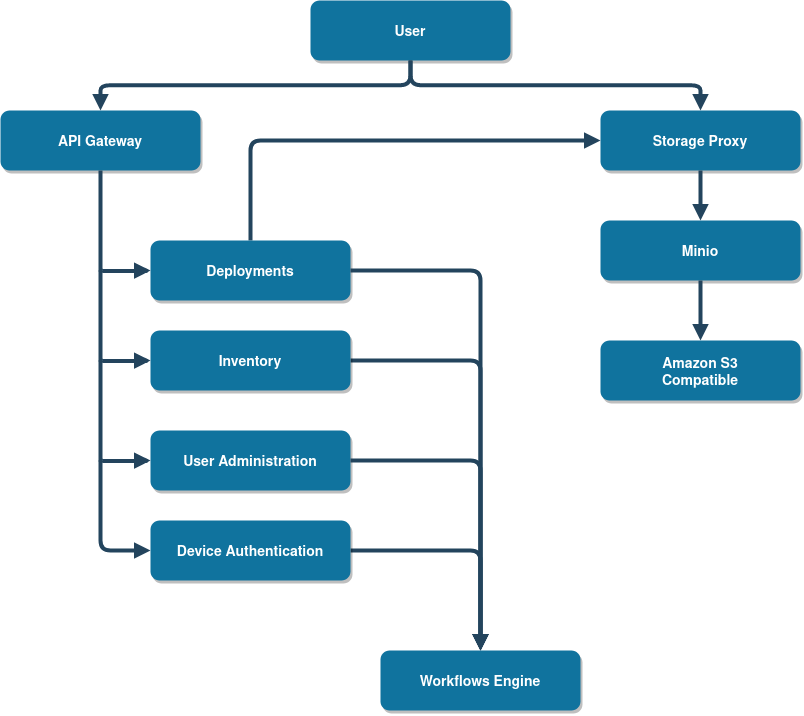
\includegraphics[scale=0.5]{images/integration-app.png}
    \caption{Mender Integration Server Architecture}
    \label{fig:mender-integration}
\end{figure}
Minio is a third-party object storage. It can either be used to serve uploaded content on its own or to proxy requests to Amazon S3 compatible cloud providers. All other services are mender application logic web services.
\newpage

\begin{figure}
    \import{gen/}{example}
    \caption{Example Code Listing}
    \label{code:example-label}
\end{figure}

Listing \ref{code:example-label} is a very good YAML file.
